\documentclass[../psets.tex]{subfiles}

\pagestyle{main}
\renewcommand{\leftmark}{Problem Set \thesection}
\setcounter{section}{3}

\begin{document}




\section{Applications of Fraction Rings}
Throughout this assignment, $R$ will denote a \emph{commutative} ring.
\begin{enumerate}
    \item \marginnote{2/1:}Let $R$ be a ring, and let $f\in R$ be an element which is not a zero divisor. Recall that we defined $R_f=D^{-1}R$ for $D=\{1,f,f^2,\dots\}$. Prove that
    \begin{equation*}
        R_f \cong R[X]/(fX-1)
    \end{equation*}
    using the universal property of the ring of fractions.
    \begin{proof}
        % We need an injective ring homomorphism $\varphi$ from $R$ to $R[X]/(fX-1)$. We also need $\varphi(D)$ to be a subset of the group of units of $R[X]/(fX-1)$. The units of $R[X]$ are the units of $R$. The units of $R[X]/(fX-1)$ are the cosets generated by the units of $R$, i.e., if $a\in R^\times$, then $a+(fX-1)$ is a unit.

        % Would our ring homomorphism be the inclusion map $a\mapsto a+(fX-1)$ for all $a\in R$? Yep. It is injective, it sends units to units. Thus, you just need to check surjectivity of $\tilde{\varphi}$.

        % A ring homomorphism from $R[X]$ to $R$ is evaluation.

        % $\varphi(f)=f+(fX-1)$. $\pi(X)=\bar{X}=X+(fX-1)$. We can define $f\bar{X}-1+(fX-1)=0+(fX-1)$, so $f\bar{X}+(fX-1)=1+(fX-1)$. 

        % Prove that $h\varphi(f)-1=0$. 

        % $f,X,1\in R[X]$, we know $f+(fX-1),X+(fX-1),1+(fX-1)\in R[X]$

        % Now let $r\in R^\times$. Then there exists $s\in R$ such that $rs=1$. It follows that
        % \begin{equation*}
        %     1+(fX-1) = \varphi(1)
        %     = \varphi(rs)
        %     = \varphi(r)\varphi(s)
        %     = [r+(fX-1)]\cdot[s+(fX-1)]
        % \end{equation*}
        % i.e., that $r+(fX-1)\in S^\times$. Therefore, since $\varphi:R\to S$ is a ring homomorphism such that $\phi(D)
        % Thus, by the universal property of the ring of fractions, 
        
        % By the universal property of the rings of fractions (UPRF), $\iota:R\to D^{-1}R$ is an injective ring homomorphism. Additionally, 
        
        % Define $\varphi:R\to S$ by
        % \begin{equation*}
        %     a \mapsto a+(fX-1)
        % \end{equation*}


        Herein, let $\bar{g}$ denote $g+(fX-1)$ for any $g\in R[X]$, and let $S$ denote $R[X]/(fX-1)$.\par
        To prove that $R_f\cong R[X]/(fX-1)$, i.e., that $D^{-1}R\cong S$, it will suffice to construct an isomorphism $\tilde{\varphi}:D^{-1}R\to S$. Per Lecture 2.2, we may define a canonical injection $i:R\to R[X]$ and a canonical surjection $\pi:R[X]\to S$.
        \par
        We now prove that the restriction $\pi|_R$ of $\pi$ to $R\cong i(R)\subset R[X]$ is injective. Suppose $\pi|_R(a)=\pi|_R(b)$ for $a,b\in R$. Then $\bar{a}=\bar{b}$, so $a\in\bar{b}$. But since $\deg(a)=0$ and $b$ is the only element of $\bar{b}$ of degree 0, we must have $a=b$, as desired.\par
        It follows that we may define an injective ring homomorphism $\varphi:R\to S$ by $\varphi=\pi|_R\circ i$. More explicitly, for any $a\in R$, we have that
        \begin{equation*}
            \varphi(a) = (\pi|_R\circ i)(a) = \pi(i(a)) = \pi(a) = \bar{a}
        \end{equation*}
        We now wish to demonstrate that $\varphi(D)\subset S^\times$. We divide into two cases ($1\in D$ and $f^n\in D$). Naturally $1\in D$, which maps to $\bar{1}\in S$ since $\varphi$ is a ring homomorphism, is a unit. To prove that every $f^n$ maps to a unit in $S^\times$, we induct on $n$. For the base case $n=1$, we have that
        \begin{align*}
            \overline{fX-1} &= \bar{0}\\
            \bar{f}\bar{X}-\bar{1} &= \bar{0}\\
            \bar{f}\bar{X} &= \bar{1}\\
            \varphi(f)\cdot\bar{X} &= \bar{1}
        \end{align*}
        Thus, $\varphi(f)\in S^\times$ by definition, as desired. Now suppose inductively that $\varphi(f^{n-1})\in S^\times$; we wish to demonstrate that $\varphi(f^n)\in S^\times$. By the induction hypothesis, there exists $\bar{b}\in S$ such that $\varphi(f^{n-1})\cdot\bar{b}=\bar{1}$. Therefore,
        \begin{align*}
            \varphi(f^n)\cdot\overline{bX} &= \varphi(f)\varphi(f^{n-1})\bar{b}\bar{X}\\
            &= \varphi(f)\bar{1}\bar{X}\\
            &= \varphi(f)\bar{X}\\
            &= \bar{1}
        \end{align*}
        as desired, where we use the base case to get from the next-to-last line to the last line above.\par
        At this point, we have proven that $\varphi:R\to S$ is an injective ring homomorphism such that $\phi(D)\subset S^\times$. Thus, we have by the universal property of rings of fractions that there exists a unique injective ring homomorphism $\tilde{\varphi}:D^{-1}R\to S$ such that $\tilde{\varphi}\circ\iota=\varphi$.\par
        To verify that $\tilde{\varphi}$ is surjective, let $\bar{g}\in S$ be arbitrary, where $g\in R[X]$. Since $R$ is a subring of $D^{-1}R$, we may consider $g\in D^{-1}R[X]$. In particular, we will be interested in $(1/f)g\in D^{-1}R[X]$ and $X-1/f\in D^{-1}R[X]$. Applying the Euclidean algorithm to the latter monic polynomial generates $q,r\in D^{-1}R[X]$ such that $(1/f)g=q(X-1/f)+r$ and, since $\deg(r)<\deg(X-1/f)=1$, $r\in D^{-1}R$. It follows that $g=q(fX-1)+rf$, so $\tilde{\varphi}(rf)=\overline{rf}=\bar{g}$ for $rf\in D^{-1}R$.\par
        Let $d$ be the denominator of $rf$. Then $drf\in R$. It follows that $\tilde{\varphi}(drf)=\tilde{\varphi}(\iota(drf))=\varphi(drf)=\overline{drf}$ so
        \begin{align*}
            \bar{d}\cdot\overline{rf} &= \tilde{\varphi}(d)\tilde{\varphi}(rf)\\
            &= \varphi(d)\tilde{\varphi}(rf)\\
            &= \bar{d}\tilde{\varphi}(rf)\\
            \overline{rf} &= \tilde{\varphi}(rf)\\
            \tilde{\varphi}(rf) &= \bar{g}
        \end{align*}
        as desired.
    \end{proof}
    \item Let $\Z[i]=\Z[X]/(X^2+1)$ denote the ring of \textbf{Gaussian integers}. Recall from class that $\Z[i]$ is a Euclidean domain with norm $N:\Z[i]\to\Zg$ defined by $N(a+bi)=a^2+b^2$.
    \begin{enumerate}[label={(\alph*)}]
        \item Let $R$ be a Euclidean domain with norm $N$ which satisfies $N(xy)=N(x)N(y)$ for all $x,y\in R$. Prove that $a\in R$ is a unit iff $N(a)=1$. (Hint: Start by computing $N(1)$.)
        \begin{proof}
            % Pick a nonzero $a\in R$. Then $N(a)>0$. It follows since
            % \begin{equation*}
            %     N(a) = N(a\cdot 1) = N(a)N(1)
            % \end{equation*}
            % by the cancellation law that $N(1)=1$.\par
            % Suppose first that $a\in R$ is a unit. Then there exists $b\in R$ such that $ab=1$. It follows that $N(a)N(b)=1$, so since $N(a),N(b)>0$, $N(a),N(b)=1$.

            Taking the hint, we will begin by computing $N(1)$. Since $1\neq 0$ and $N$ is a positive norm by assumption, $N(1)>0$. Additionally, since $\Z$ is an integral domain, we can use the cancellation law between the following equations.
            \begin{align*}
                N(1\cdot 1) &= N(1)\\
                N(1)N(1) &= N(1)\cdot 1\\
                N(1) &= 1
            \end{align*}
            Having computed $N(1)$, we now begin the argument in earnest.\par
            Suppose first that $a\in R$ is a unit. Then there exists $b\in R$ such that $ab=1$. It follows that
            \begin{align*}
                N(ab) &= N(1)\\
                N(a)N(b) &= 1
            \end{align*}
            Thus, $N(a)=\pm 1$, but since $N(a)\in\Zg$, we must have
            \begin{equation*}
                N(a) = 1
            \end{equation*}
            as desired.\par
            Now suppose that $N(a)=1$. Since $R$ is an ED and $a\neq 0$, we know that there exist $q,r\in R$ such that $1=qa+r$ and $N(a)>N(r)$. But since $N(1)=1$, we must have $N(r)=0$ or $r=0$. Therefore, $1=qa$, so $a$ is a unit, as desired.
        \end{proof}
        \item Using part (a), find the units in $\Z[i]$.
        \begin{proof}
            Let $a+bi\in\Z[i]$ be a unit. Then $1=N(a+bi)=a^2+b^2$. The four possible solutions over $\Z$ are $(a,b)=(\pm 1,0)$ and $(a,b)=(0,\pm 1)$. Therefore, the units of $\Z[i]$ are
            \begin{equation*}
                \boxed{\pm 1,\pm i}
            \end{equation*}
        \end{proof}
        \item Prove that $\Frac(\Z[i])=\Q[i]$.
        \begin{proof}
            % Kinda separate; just use a bidirectional inclusion proof. Might be able to use part (b) a bit??

            To prove that $\Frac(\Z[i])=\Q[i]$, it will suffice to use a bidirectional inclusion argument.\par
            Suppose first that
            \begin{equation*}
                \frac{a+bi}{c+di} \in \Frac(\Z[i])
            \end{equation*}
            Then by the laws of multiplication on the field of fractions and on $\Z[i]$, we have that
            \begin{equation*}
                \frac{a+bi}{c+di} = \frac{a+bi}{c+di}\cdot\frac{c-di}{c-di}
                = \frac{(a+bi)(c-di)}{(c+di)(c-di)}
                = \frac{(ac+bd)+(bc-ad)i}{c^2+d^2}
                = \frac{ac+bd}{c^2+d^2}+\frac{bc-ad}{c^2+d^2}i
            \end{equation*}
            Since $a+bi,c+di\in\Z[i]=\{\alpha+\beta i\mid \alpha,\beta\in\Z\}$ by the definition of $\Frac(\Z[i])$, we know that $a,b,c,d\in\Z$. Thus,
            \begin{equation*}
                \frac{ac+bd}{c^2+d^2},\frac{bc-ad}{c^2+d^2} \in \Q
            \end{equation*}
            and hence
            \begin{equation*}
                \frac{a+bi}{c+di} = \frac{ac+bd}{c^2+d^2}+\frac{bc-ad}{c^2+d^2}i \in \{\alpha+\beta i\mid \alpha,\beta\in\Q\}=\Q[i]
            \end{equation*}
            as desired.\par
            Now suppose that
            \begin{equation*}
                \frac{a}{b}+\frac{c}{d}i \in \Q[i]
            \end{equation*}
            Then by the laws of addition and multiplication on $\Q[i]$ and on $\Z[i]$, we have that
            \begin{equation*}
                \frac{a}{b}+\frac{c}{d}i = \frac{a}{b}+\frac{c}{d}\frac{i}{1}
                = \frac{a}{b}+\frac{ci}{d1}
                = \frac{a}{b}+\frac{ci}{d}
                = \frac{ad+bci}{bd}
                = \frac{ad+bci}{bd+0i}
            \end{equation*}
            Since $a/b,c/d\in\Q$, $a,b,c,d\in\Z$. Thus, $ad,bc,bd,0\in\Z$ so $ad+bci,bd+0i\in\Z[i]$. Additionally, since $b,d\in\Z\setminus\{0\}$ by hypothesis, $bd+0i\neq 0$ as well. Therefore,
            \begin{equation*}
                \frac{a}{b}+\frac{c}{d}i = \frac{ad+bci}{bd+0i} \in \Frac(\Z[i])
            \end{equation*}
            as desired.
        \end{proof}
    \end{enumerate}
    \item 
    \begin{enumerate}[label={(\alph*)}]
        \item For $a,b\in\Z$, prove that $a^2-2b^2=0$ iff $a=b=0$.
        \begin{proof}
            % $\Z$ is a UFD, and $a^2$ and $2b^2$ necessarily have different factorizations.

            % Suppose for the sake of contradiction that there exist nonzero integers $a,b$ such that $a^2=2b^2$. Then there exists $a,b$ of smallest value. Since $a^2=2b^2$, $a^2$ is an even number. Thus, $a$ is an even number, and hence $a=2c$. It follows that $2c^2=b^2$, contradicting our hypothesis that $a,b$ were minimal. Then $2a^2=(2b)^2$

            % $a/b=\sqrt{2}$ where $a/b$ is a rational number and $\sqrt{2}$ is irrational, a contradiction.\par
            % Obviously, if $a=b=0$, then $a^2-2b^2=0^2-2\cdot 0^2=0$, as desired.


            For the forward direction, let that $a,b\in\Z$ satisfy $a^2-2b^2=0$. Suppose for the sake of contradiction that either $a$ or $b$ is nonzero. It follows by the derived equality $a^2=2b^2$ that they are both nonzero. Thus, $a/b$ is a well-defined element of $\Q$. However, we have that
            \begin{align*}
                a^2-2b^2 &= 0\\
                a^2 &= 2b^2\\
                \frac{a^2}{b^2} &= 2\\
                \frac{a}{b} &= \sqrt{2}
            \end{align*}
            i.e., that a rational number equals an irrational number, a contradiction. Therefore, $a=b=0$.\par
            For the reverse direction, let $a=b=0$. Then
            \begin{equation*}
                a^2-2b^2 = 0^2-2\cdot 0^2 = 0
            \end{equation*}
            as desired.
        \end{proof}
        \item Prove that $\Q[\sqrt{2}]=\Q[X]/(X^2-2)$ is a field.
        \begin{proof}
            % Check all of the field axioms using multiplication in $\Q$.
            % $\Q$ is a field.
            % $\Q[X]$ is a PID.

            % To prove that the given ring is a field, it will suffice to show that $(X^2-2)$ is a maximal ideal.


            To prove that $\Q[\sqrt{2}]=\Q[X]/(X^2-2)$ is a field, it will suffice to show that its additive and multiplicative identites are distinct and that every element is a unit. Let's begin.\par
            $\Q[X]/(X^2-2)$ inherits addition and multiplication from $\Q[X]$, except now modulo $X^2-1$. Thus, the additive and multiplicative identities of $\Q[X]/(X^2-2)$ are the (distinct) images of those in $\Q[X]$ under the relevant canonical surjection.\par
            Now let $a+b\sqrt{2}\in\Q[\sqrt{2}]$ be arbitrary and nonzero. Then $a$ or $b$ is nonzero. It follows by part (a) that $a^2-2b^2\neq 0$, and hence
            \begin{equation*}
                \frac{a}{a^2-2b^2}-\frac{b}{a^2-2b^2}\sqrt{2} \in \Q[\sqrt{2}]
            \end{equation*}
            is well-defined. By the law of multiplication in $\Q[\sqrt{2}]$, it follows that
            \begin{equation*}
                \left( a+b\sqrt{2} \right)\left( \frac{a}{a^2-2b^2}-\frac{b}{a^2-2b^2}\sqrt{2} \right) = \frac{\left( a+b\sqrt{2} \right)\left( a-b\sqrt{2} \right)}{a^2-2b^2}
                = \frac{a^2-b^2\sqrt{2}^2}{a^2-2b^2}
                = \frac{a^2-2b^2}{a^2-2b^2}
                = 1
            \end{equation*}
            as desired. Note that as in Q4.1, we can prove that $\sqrt{2}$ is the solution to $X^2-2=0$, i.e., an object $X$ such that $X^2=2$. This is what rigorously allows us to simplify the above equation, not any intuitive or notationally implied notion of $\sqrt{2}$.
        \end{proof}
    \end{enumerate}
    \item Let $D$ be a multiplicative subset of an integral domain $R$. Now $R$ is a subring of $D^{-1}R$. Let $J$ be an ideal of $D^{-1}R$. Put $I=R\cap J$.
    \begin{enumerate}[label={(\alph*)}]
        \item Is $I$ an ideal of $R$?
        \begin{proof}
            % Prove or disprove from the definition.
            % $J$ is closed under multiplication by elements of $D^{-1}R$. This includes elements of $R$, so $J$ is closed under multiplication by elements of $R$.
            % Pretty sure that's true.

            \fbox{Yes} $I$ is an ideal of $R$.\par
            Since $R,J$ are both additive subgroups of $D^{-1}R$, $R\cap J$ is an additive subgroup of $D^{-1}R$. Additionally, since $R\cap J\subset R$, $R\cap J$ must be an additive subgroup of $R$.\par
            Now let $x\in I$ and $r\in R$ be arbitrary. Since $x\in I$, $x\in R$ and $x\in J$. It follows from the former statement and the fact that $R$ is an ideal of $R$ that $rx\in R$. It follows from the latter statement and the fact that $J$ is an ideal of $D^{-1}R$ that $rx\in J$. Therefore, $rx\in R\cap J=I$, as desired.
        \end{proof}
        \item Prove that if $I\neq R$, then $I\cap D=\emptyset$.
        \begin{proof}
            % Since $R$ is an integral domain, $D^{-1}R$ is a field. Since the only ideals of a field are $\{0\}$ and $D^{-1}R$, and $I\neq R$ implies $J\neq R$, then $J=\{0\}$ and hence $I=R\cap J=\{0\}$. It follows since $0\notin D$ by definition that $I\cap D=\emptyset$, as desired.

            % Suppose $J\neq\{0\}$. Let $a/b\in J$ be nonzero, and take $a,b$ to be relatively prime. We divide into two cases ($a\in D$ and $a\notin D$). If $a\in D$, then $b/a\in D^{-1}R$. Hence, $1=a/b\cdot b/a\in J$. Thus, $J=R$, so $I=R\cap R=R$. But this contradicts our hypothesis that $I\neq R$, so we don't have to worry about this case. Now suppose $a\notin D$. Then $(a)\neq R$. $a\in J$ and $a\in I$


            Suppose for the sake of contradiction that there exists $x\in I\cap D$. Then $x\in I$ and $x\in D$. It follows from the latter statement that $1/x\in D^{-1}R$. It follows from the former statement that $x\in R$ and $x\in J$. Since $J$ is an ideal of $D^{-1}R$ (hence is closed under multiplication by elements of $D^{-1}R$) and $x\in J$, we have in particular that
            \begin{equation*}
                \frac{1}{x}\cdot x = \frac{x}{x} = 1 \in J
            \end{equation*}
            It follows that $J=D^{-1}R$. Consequently, since $R\subset D^{-1}R$, we have that $I=R\cap D^{-1}R=R$. This contradicts the hypothesis that $I\neq R$.
        \end{proof}
        \item Let $b\in J$. Is it true that $b=d^{-1}a$ for some $d\in D$ and $a\in I$?
        \begin{proof}
            \fbox{Yes} it is true.\par
            Since $b\in J$, we know that $b\in D^{-1}R$. It follows that we may write $b=a/d$ for some $a\in R$ and $d\in D$. Since $J$ is an ideal and $d\in D\subset R\subset D^{-1}R$, we know that $a=db\in J$. Combining the facts that $a\in R$ and $a\in J$, we can determine that $a\in R\cap J=I$, as desired.
        \end{proof}
        \item Prove that if $I$ is an ideal in $R$, then $I^e=\{s^{-1}x\in D^{-1}R\mid s\in D,\ x\in I\}$ is an ideal in $D^{-1}R$.
        \begin{proof}
            To prove that $I^e$ is an ideal, it will suffice to show that $(I^e,+)\leq(D^{-1}R,+)$ and $a/b\cdot x/s\in I^e$ for all $a/b\in D^{-1}R$ and $x/s\in I^e$.\par
            First, we will show that $(I^e,+)$ is a subgroup. By definition, it is a subset of $D^{-1}R$. Since $0\in I$ and $D$ is nonempty, the identity $0/d\in I^e$. Associativity follows from the containing group. And closure follows from that of $I$ (under multiplication by elements of $R$ and addition) and that of $D$ (under multiplication by elements of $D$): If $x_1/s_1,x_2/s_2\in I^e$, then
            \begin{equation*}
                \frac{x_1}{s_1}+\frac{x_2}{s_2} = \frac{x_1s_2+x_2s_1}{s_1s_2} \in I^e
            \end{equation*}
            as desired.\par
            Now we show closure under multiplication. Let $x/s\in I^e$ and $a/b\in D^{-1}R$ be arbitrary. Since $x\in I$ and $a\in R$, $xa\in I$. Since $s,b\in D$, $sb\in D$. Therefore,
            \begin{equation*}
                \frac{x}{s}\cdot\frac{a}{b} = \frac{xa}{sb} \in I^e
            \end{equation*}
            as desired.
        \end{proof}
        \item Using part (c), prove that if $J$ is an ideal of $D^{-1}R$, then $J=(R\cap J)^e$. Therefore, we have a surjective map of sets
        \begin{equation*}
            \{\text{Ideals in }R\} \to \{\text{Ideals in }D^{-1}R\}
        \end{equation*}
        given by $I\mapsto I^e$. Note that the right inverse is given by $J\mapsto R\cap J$. Is this map a bijection?
        \begin{proof}
            To prove that $J=(R\cap J)^e$, we will use a bidirectional inclusion proof. Suppose first that $b\in J$. Then by part (c), $b=d^{-1}a$ for some $d\in D$ and $a\in I$. Therefore, by the definition of $(R\cap J)^e$, $b\in(R\cap J)^e$. Now suppose that $d^{-1}a\in(R\cap J)^e$ Then $a\in R\cap J$, so $a\in J$. It follows since $J$ is an ideal of $D^{-1}R$ and $1/d\in D^{-1}R$ that $a/d=d^{-1}a\in J$, as desired.\par
            % \fbox{Yes} this map is a bijection. To prove that the given right inverse is also a left inverse, take $I\mapsto I^e\mapsto R\cap I^e$; our goal is to prove that $I=R\cap I^e$. Let $x\in I$ be arbitrary. Then $x\in R$. Additionally, taking $1\in D$, we have that $x=x/1\in I^e$. Therefore, $x\in R\cap I^e$. In the other direction, let $x\in R\cap I^e$ be arbitrary. Since $x\in I^e$, we have that $x=a/s$ for some $a\in I$ and $s\in D$. Since $x\in R$, we must have $s=1$ and therefore $x=a/1=a\in I$, as desired.
            \fbox{No} this map is not a bijection. Counterexample: Let $R,D$ be defined as in Q5. Consider $(3)$. Since $3\in D$, $1=3/3\in(3)^e$. Thus, $(3)^e=D^{-1}R$. It follows that $\Z^e=(3)^e$ even though $\Z\neq(3)$.
        \end{proof}
        \item If $R$ is a PID, is $D^{-1}R$ a PID?
        \begin{proof}
            % Let $I$ be an ideal in $R$. Then $I=(a)$ for some $a\in R$. It follows that $I^e$ is an ideal in $D^{-1}R$. $a\in I^e$ is a generator? Let $x/s$ be arbitrary. We know $x=ab$. $x/s=a\cdot(b/s)$. 

            \fbox{Yes.}\par
            Let $J\in D^{-1}R$ be an arbitrary ideal. Per part (e), there exists an ideal $I\subset R$ such that $J=I^e$. Since $R$ is a PID, $I=Ra$ for some $a\in I$. Additionally, as per the definition of the extension map, $a=a/1\in I^e=J$. We will now prove that $I^e=D^{-1}Ra$. By definition, $D^{-1}Ra\subset I^e$. In the other direction, let $x/s\in I^e$ be arbitrary. Since $x\in I$, $x=ab$ for some $b\in R$. Moreover, $b/s\in D^{-1}R$, so $x/s=(b/s)\cdot a\in D^{-1}Ra$, as desired.
        \end{proof}
    \end{enumerate}
    \item 
    \begin{enumerate}[label={(\alph*)}]
        \item Let $D=\{n\in\Z:2\nmid n\}$. Recall that we defined
        \begin{equation*}
            \Z_{(2)} = D^{-1}R
            = \{a/b\in\Q:2\nmid b\}
        \end{equation*}
        Write down all of the ideals in $\Z_{(2)}$. You can use the fact that the ideals in $\Z$ are $(n)=n\Z$ for $n\in\Z$, and the previous question. Which of these ideals are maximal? For each maximal ideal $M\in\Z_{(2)}$, what is the field $\Z_{(2)}/M$?
        \begin{proof}
            % The maximal ideals are \fbox{those for which $n$ is prime.}
            % Cly 14: Maximal are prime.
            % Let $(n)^e\subset\Z_{(2)}$ be an arbitrary prime ideal. Suppose for the sake of contradiction that there exists some $m\in\Z$ such that $(n)^e\subsetneq(m)^e\subsetneq\Z_{(2)}$. It follows by the former inclusion that $n\in(m)^e$ and hence $m\mid n$.

            % $n\in(m)^e$, so $n=d^{-1}a$ for some $a\in(m)$ $a=bm$. $dn=bm$. $n=(b/d)\cdot m$.
            
            % We prove the implication both ways. First, let $n\in\Z$ is prime. Then $(n)$ is a prime ideal in $\Z$. It follows that $(n)^e$ is a prime ideal in $\Z_{(2)}$: Let $a,b\in\Z_{(2)}$ be such that $ab\in(n)^e$. Then $ab=d^{-1}c$ for some $c\in(n)$ and $d\in D$. $c=ne$. $ab=ne/d$. WTS: $a=d^{-1}f$
            
            % Suppose for the sake of contradiction that there exists $m\in\Z$ such taht

            % Alternatively, $\Z_{(2)}/(n)^e$ is an integral domain. Let $\bar{a}\in\Z_{(2)}/(n)^e$ be arbitrary. Then $\bar{a}=a+(n)^e$.

            % The set of all fractions in $\Q$ with denominator coprime to 2. Is it $\Z/2\Z$? Perhaps isomorphic to the set of all $1/d$ plus 0, or $D\cup\{0\}$.

            % Define $\pi:\Z/2\Z\to\Z_{(2)}/(2)^e$ analogously to the canonical surjection, i.e., by $\pi(a)=a+(2)^e$ ($a=0,1$). By the definitions of addition and multiplication on a ring (i.e., componentwise), it follows that $\pi$ is a ring homomorphism.\par
            % For injectivity, suppose $\pi(a)=\pi(b)$. Then $a+(2)^e=b+(2)^e$, so $b=a+2c/d$ for some $c\in\Z$ and $d\in D$.


            Since the ideals in $\Z$ are $(n)=n\Z$ for all $n\in\Z$, Q4.4e implies that the set of ideals of $\Z_{(2)}$ is the image of $\{(n)\mid n\in\Z\}$ under $I\mapsto I^e$. However, many of these are equivalent. In particular, if $n$ is divisible by any numbers other than 2, you will be able to multiply $n$ by the product of those numbers to reduce the magnitude of the generator down to a power of 2. Therefore, the set of all ideals in $\Z_{(2)}$ is
            \begin{equation*}
                \boxed{\{(2^n)^e\mid n\in\Zg\}\cup\{0\}}
            \end{equation*}
            Among these ideals,
            \begin{equation*}
                \boxed{\text{Only }(2)^e\text{ is maximal.}}
            \end{equation*}
            To prove this, we will show that every ideal $(n)^e\in\Z_{(2)}$ is either equal to $\Z_{(2)}$ or is contained in $(2)^e$. Let's begin. Let $(n)^e\subset\Z_{(2)}$ be arbitrary. We divide into two cases ($2\nmid n$ and $2\mid n$). If $2\nmid n$, then $n\in D$. It follows by its definition that $1=n/n\in(n)^e$. Therefore, $(n)^e=R$. If $2\mid n$, then $n=2^m\cdot r$ for some $m\geq 1$ and $r$ coprime to $2$. Let $a/d\in(n)^e$ be arbitrary. Then $a\in(n)$ and $d\in D$. It follows that $n\mid a$, i.e., that $2\mid a$. Thus, $a=2b\in(2)$. Therefore, $a/d\in(2)^e$, so $(n)^e\subset(2)^e$, as desired.\par
            Finally, we will prove that
            \begin{equation*}
                \boxed{\Z_{(2)}/(2)^e \cong \Z/2\Z}
            \end{equation*}
            To do so, it will suffice to show that for any $a/d\in\Z_{(2)}$, we either have
            \begin{align*}
                \frac{a}{d}+(2)^e &= 0+(2)^e&
                \frac{a}{d}+(2)^e &= 1+(2)^e
            \end{align*}
            Since $\Z$ is an ED and $2\neq 0$, we know that there exist $b,c\in\Z$ such that $a=2b+c$ and $|c|<|2|=2$ (i.e., $c\in\{0,\pm 1\}$). We now divide into three cases. If $c=0$, then $a=2b$ and hence
            \begin{equation*}
                \frac{a}{d} = \frac{2b}{d} \in (2)^e
            \end{equation*}
            so $a/d+(2)^e=0+(2)^e$. If $c=1$, then
            \begin{equation*}
                \frac{a}{d} = \frac{1}{d}+\frac{2b}{d}
            \end{equation*}
            so $a/d\in 1/d+(2)^e$. Additinally, since $2\nmid d$ by hypothesis, $2\mid d-1$ and hence $\pm(d-1)/d\in(2)^e$. It follows that
            \begin{equation*}
                \frac{1}{d} = \frac{1}{d}+\frac{d-1}{d}-\frac{d-1}{d}
                = 1+-\frac{d-1}{d}
                \in 1+(2)^e
            \end{equation*}
            Therefore, $a/d\in 1+(2)^e$, as desired. The case $c=-1$ is analogous to the case $c=1$.
        \end{proof}
        \item Let $D=\{2^n\mid n\in\Zg\}$ and let $R=D^{-1}\Z$. Write down the ideals in $R$. Which of these ideals are maximal?
        \begin{proof}
            % Let $a/d\in I$ be arbitrary. It follows that $a\in I$. Q4.4e: $I=(n)^e$. $(n)^e=(n)$.
            
            % Let $n$ be the smallest nonzero numerator present in any element of $I$. It follows that $(n,2)=1$ since if not, then $(n/2)/1$ would give rise to a smaller nonzero numerator. Moreover, we can prove that $I=(n)$, as follows.

            The set of all ideals in $R$ is
            \begin{equation*}
                \boxed{\{(n):(n,2)\leq 1\}}
            \end{equation*}
            By definition, $(n)$ is an ideal in $R$. Now suppose that $I$ is an arbitrary ideal in $R$. By Q4.4e and the fact that the ideals of $\Z$ are of the form $(n)$ for some $n\in\Z$, $I=(n)^e$. To verify that $(n)^e=D^{-1}\Z n=(n)$, first let $a/2^m\in(n)^e$. Then since $1/2^m\in R$, $a/2^m=a\cdot(1/2^m)\in(n)$. Now let $na/2^m\in(n)$. Then since $na\in(n)$, $na/2^m\in(n)^e$. Now suppose $(n,2)>1$. Then $2\mid n$ and hence $(n/2)/1\in(n)$, contradicting the assumption that the generator $n$ is the smallest element of $(n)$.\par
            The maximal ideals in $R$ are the subset of the above consisting of all prime ideals, i.e.,
            \begin{equation*}
                \boxed{\{(n):n\text{ is prime}\}}
            \end{equation*}
            We know that every maximal ideal is prime. In the other direction, suppose $(n)$ is a prime ideal. Now suppose for the sake of contradiction that $(n)\subsetneq(m)\subsetneq R$. It follows that $n\in(m)$. Thus, $n=(a/b)m$ for some $a/b\in R$. Consequently, since $(n)$ is a prime ideal, $m\in(n)$ or $a/b\in(n)$. We now divide into two cases. If $m\in(n)$, then $(m)\subset(n)$, a contradiction. If $a/b\in(n)$, then $a/b=n\cdot(c/d)$. Combining this with the result that $n=(a/b)m$, we have that
            \begin{align*}
                n &= \frac{a}{b}\cdot m\\
                &= \frac{nc}{d}\cdot m\\
                1 &= \frac{c}{d}\cdot m
            \end{align*}
            But then $1\in(m)$, and hence $(m)=R$, a contradiction.
        \end{proof}
    \end{enumerate}
    \item 
    \begin{enumerate}[label={(\alph*)}]
        \item Define $M_2:\{\text{commutative rings}\}\to\{\text{sets}\}$ by
        \begin{equation*}
            M_2(R) = \left\{
                \begin{pmatrix}
                    a & b\\
                    c & d\\
                \end{pmatrix}
                \mid a,b,c,d\in R
            \right\}
        \end{equation*}
        Show that for any $R$, there is a natural bijection between the set $M_2(R)$ and the set $S_1$ of ring homomorphisms between $\Z[X,Y,Z,W]$ and $R$. Note that notationally,
        \begin{equation*}
            S_1 = \text{Hom}_\text{ring}(\Z[X,Y,Z,W],R)
        \end{equation*}
        One sometimes says that $\Z[X,Y,Z,W]$ represents the function $M_2$.
        \begin{proof}
            % Characteristic polynomial function??
            Define $\psi:M_2(R)\to S_1$ by
            \begin{equation*}
                \begin{pmatrix}
                    a & b\\
                    c & d\\
                \end{pmatrix}
                \mapsto \ev_{(a,b,c,d)}
            \end{equation*}
            We know from class that every evaluation function is a ring homomorphism. Thus, $\ev_{(a,b,c,d)}$ does lie in the correct set.\par
            \underline{Injectivity}: Suppose
            \begin{equation*}
                \psi\left[
                    \begin{pmatrix}
                        a_1 & b_1\\
                        c_1 & d_1\\
                    \end{pmatrix}
                \right] = \psi\left[
                    \begin{pmatrix}
                        a_2 & b_2\\
                        c_2 & d_2\\
                    \end{pmatrix}
                \right]
            \end{equation*}
            Then $\ev_{(a_1,b_1,c_1,d_1)}=\ev_{(a_2,b_2,c_2,d_2)}$. It follows that
            \begin{equation*}
                a_1 = \ev_{(a_1,b_1,c_1,d_1)}(X) = \ev_{(a_2,b_2,c_2,d_2)}(X) = a_2
            \end{equation*}
            Similar statements hold for $b,c,d$. Thus, since $x_1=x_2$ ($x\in\{a,b,c,d\}$), we have that
            \begin{equation*}
                \begin{pmatrix}
                    a_1 & b_1\\
                    c_1 & d_1\\
                \end{pmatrix}
                =
                \begin{pmatrix}
                    a_2 & b_2\\
                    c_2 & d_2\\
                \end{pmatrix}
            \end{equation*}
            as desired.\par
            \underline{Surjectivity}: Let $\varphi\in S_1$ be arbitrary. Suppose $\varphi(X)=a$, $\varphi(Y)=b$, $\varphi(Z)=c$, and $\varphi(W)=d$. Since any polynomial in $\Z[X,Y,Z,W]$ is a $\Z$-linear combination of $X,Y,Z,W$ and $\varphi$ respects these addition and multiplication operations, we have that for any $f\in\Z[X,Y,Z,W]$,
            \begin{equation*}
                \varphi(f) = f(a,b,c,d) = \ev_{(a,b,c,d)}(f)
            \end{equation*}
            Therefore,
            \begin{equation*}
                \psi\left[
                    \begin{pmatrix}
                        a & b\\
                        c & d\\
                    \end{pmatrix}
                \right] = \ev_{(a,b,c,d)} = \varphi
            \end{equation*}
            as desired.
        \end{proof}
        \item (\textbf{You do not need to turn in part (b)}, but you are encouraged to think about it.)\par
        Actually, $M_2(R)$ can be naturally given a ring structure: Addition and multiplication are defined using the same procedure as $M_2(\R)$ (or with any other field you may have seen). Hence, it makes sense to talk about the units of $M_2(R)$.\par
        Define the set $GL_2(R)$ to be the units of $M_2(R)$, i.e.,
        \begin{equation*}
            GL_2(R) = M_2(R)^\times
        \end{equation*}
        Show that for any $R$, there is a natural bijection between $GL_2(R)$ and the set $S_2$ defined by
        \begin{equation*}
            S_2 = \text{Hom}_\text{ring}(\Z[X,Y,Z,W]_{XW-YZ},R)
        \end{equation*}
        Note that $\Z[X,Y,Z,W]_{XW-YZ}$ denotes the \textbf{localization} of $\Z[X,Y,Z,W]$ by the multiplicative set generated by $XW-YZ$ (that is, the multiplicative set $(1,XW-YZ,(XW-YZ)^2,\dots)$). (Hint: Use the universal property.)\par
        One sometimes says $\Z[X,Y,Z,W]_{XW-YZ}$ represents the function $GL_2$.
        % \begin{proof}
        %     XW-YZ is like the determinant.
        % \end{proof}
    \end{enumerate}
    \item Let $\Q(X)$ denote the field of fractions of $\Q[X]$. By the universal property of a polynomial ring, we know that giving a ring homomorphism $\varphi:\Q[X]\to\R$ is equivalent to choosing an element $r\in\R$ and setting $\varphi(X)=r$. Which ring homomorphisms $\varphi:\Q[X]\to\R$ extend to ring homomorphisms $\tilde{\varphi}:\Q(X)\to\R$? These ring homomorphisms should satisfy the following commutative diagram.
    \begin{center}
        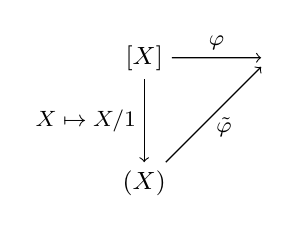
\begin{tikzpicture}[scale=1.6]
            \small
            \node (pols) at (0,1) {$\Q[X]$};
            \node (frcs) at (0,0) {$\Q(X)$};
            \node (R)    at (1,1) {$\R$};
    
            \footnotesize
            \draw [->] (pols) -- node[left]            {$X\mapsto X/1$}    (frcs);
            \draw [->] (frcs) -- node[below right=-2pt]{$\tilde{\varphi}$} (R);
            \draw [->] (pols) -- node[above]           {$\varphi$}         (R);
        \end{tikzpicture}
    \end{center}
    \begin{proof}
        % It follows that $\varphi=\ev_r$. 

        % Those for which $r$ is irrational. If $r$ is irrational, then $f(r)\neq 0$ for any $f\in\Q[X]$. $r$ must be \emph{transcendental}.


        We can prove that the set of ring homomorphisms $\varphi$ which extend to the field of rational functions over $\Q$ is equal to
        \begin{equation*}
            \boxed{\{\varphi:\varphi(X)\text{ is a real transcendental number}\}}
        \end{equation*}
        Let $\varphi$ be an element of the above set. Since $\varphi(X)=r$ is transcendental, $\varphi(f)=\ev_r(f)\neq 0$ for any $f\in\Q[X]$. (Note that a similar argument to the surjectivity one used in Q4.6a can justify that $\varphi=\ev_r$.) It follows that if we extend $\varphi$ to $\Q(X)$ by keeping the evaluation definition (recall that evaluation is always a ring homomorphism), then for any rational function $f/g\in\Q(X)$,
        \begin{equation*}
            \tilde{\varphi}\left( \frac{f}{g} \right) = \left( \frac{f}{g} \right)(r) = \frac{f(r)}{g(r)}
        \end{equation*}
        where, as established, $g(r)$ is nonzero and hence $\tilde{\varphi}(f/g)$ is well-defined.\par
        Now suppose that $\varphi:\Q[X]\to\R$ is a ring homomorphism that extends to a ring homomorphism $\tilde{\varphi}:\Q(X)\to\R$. Let $\tilde{\varphi}(X)=\varphi(X)=r$. Then as per Q4.6a, $\tilde{\varphi}=\ev_r$. Since $\tilde{\varphi}$ is a ring homomorphism, $\tilde{\varphi}(f/g)$ is well-defined for every $f\in\Q[X]$ and $g\in\Q[X]-\{0\}$. In particular, we must have $0\neq\tilde{\varphi}(g)=\ev_r(g)=g(r)$ for all such $g$. It follows by definition that $r$ is a real transcendental number.
    \end{proof}
    \item $F$ is a field. Let $R$ be the smallest subring of $F[X]$ such that (a) $F\subset R$ and (b) both $X^2$ and $X^3$ belong to $R$.
    \begin{enumerate}[label={(\alph*)}]
        \item Use the identity $(X^2)^3=(X^3)^2$ to deduce that $R$ is \emph{not} a UFD.
        \begin{proof}
            % We have that $R=(X^2,X^3)\cup F$. $X^2,X^3$ are irreducible. $X^6=(X^2)^3=(X^3)^2$. But these factorizations have different lengths, so $R$ cannot be a UFD.

            % The smallest subring of $F[X]$ containing $F$ is $F$. The smallest subring of $F[X]$ containing $X^2$ and $X^3$ is $(X^2,X^3)$. Thus, the smallest subring of $F[X]$ containing both is $R=F+(X^2,X^3)$.

            % for some units $u,v$ such that $uv=1$.

            % Suppose for the sake of contradiction that $X^2$ and $X^3$ are reducible. Then by Lecture 5.2, there exists $g\in R$ such that $\deg(g)=1$ and $g\mid X^2$.


            Suppose for the sake of contradiction that $X^2$ is reducible. Then $X^2=ab$ where $a,b\notin R^\times=F^\times$. It follows since they aren't units that $\deg(a),\deg(b)\geq 1$. But since $\deg(a)+\deg(b)=\deg(ab)=2$, it must be that $\deg(a)=\deg(b)=1$. Thus, $a=c_1X+d_1$ and $b=c_2X+d_2$. It follows that
            \begin{align*}
                X^2 &= ab\\
                1X^2+0X+0 &= c_1c_2X^2+(c_1d_2+c_2d_1)X+d_1d_2
            \end{align*}
            so
            \begin{align*}
                c_1c_2 &= 1&
                d_1d_2 &= 0
            \end{align*}
            Then $c_1,c_2\in R^\times=F^\times$ and $d_1=d_2=0$. It follows that $X=c_1c_2X\in R$, and hence $R=F[X]$ by the construction from Lecture 1.2. However, this contradicts the hypothesis that $R$ is the smallest subring of $F[X]$ containing $F,X^2,X^3$ since $F+(X^2,X^3)$ is an example of a smaller subring of $F[X]$ containing $F,X^2,X^3$. Therefore, $X^2$ is irreducible in $R$.\par
            A similar argument can show that $X^3$ is irreducible in $R$.\par
            It follows that two factorizations of $X^6$ are $(X^2)^3$ and $(X^3)^2$. But since these factorizations have different lengths, they are not equivalent. Therefore, $R$ is not a UFD, as desired.
        \end{proof}
        \item Exhibit an ideal $I$ of $R$ that is not a principal ideal.
        \begin{proof}
            Take
            \begin{equation*}
                \boxed{I = (X^2,X^3)}
            \end{equation*}
            Since both generators are irreducible by part (a), their greatest common divisor is necessarily a unit. Thus, since $(X^2,X^3)$ only consists of polynomials of degree greater than or equal to 2 (i.e., objects that are not units), no element of it can generate both extant generators. Therefore, $(2,X)$ is not principal.
        \end{proof}
    \end{enumerate}
    \item Mimic Euclid's proof of the infinitude of primes in $\Z$ to show that $F[X]$ has infinitely many primes for every field $F$.
    \begin{proof}
        % Then $(f_1),\dots,(f_r)$ are all prime ideals. We will now prove that $(f_1\cdots f_r+1)$ is a prime ideal. Since
        % \begin{equation*}
        %     f_1\cdots f_r+1 = f_i\cdot\prod_{\substack{j=1\\j\neq i}}^rf_j+1
        % \end{equation*}
        
        Suppose for the sake of contradiction that $\{f_1,\dots,f_r\}$ is the set of all primes in $F[X]$. Since $F[X]$ is an ED, it is a PID. Thus, the primes and irreducibles coincide. Likewise, $F[X]$ being an ED makes it a UFD. Thus, the element $f_1\cdots f_r+1$ (for example) has a unique factorization in terms of $f_1,\dots,f_r$. In particular, since each $f_i$ irreducible and hence not a unit, $\deg(f_i)\geq 1$ ($i=1,\dots,r$). This means that $\deg(f_1\cdots f_r+1)\geq r$ so $f_1\cdots f_r+1$ is not a unit. It follows that there exists at least one $f_i$ such that $f_i\mid f_1\cdots f_r+1$. Additionally, $f_i\mid f_1\cdots f_r$. Thus, $f_i\mid f_1\cdots f_r+1-f_1\cdots f_r=1$. Therefore, $f_i$ is a unit, a contradiction.
    \end{proof}
    \item Let $R$ be an integral domain and let $d$ be the degree of a nonzero $f\in R[X]$. Prove that $\{a\in R\mid f(a)=0\}$ is finite. \emph{Hint}: Case 1 --- first prove this when $R$ is a field. Case 2 --- reduce to case 1 by looking at the fraction field of $R$.
    \begin{proof}
        % This is the roots of $f$.

        % Let $A=\{a\in R\mid f(a)=0\}$. Suppose for the sake of contradiction that $|A|>d$. Choose a subset $\{a_0,\dots,a_d\}\subset A$ of cardinality $d+1$. Since $f\in R[X]$ and $X-a_0$ is a monic polynomial, the Euclidean algorithm implies that $f=q_0(X-a_0)+r_0$ for some $q_0,r_0\in R[X]$ with $\deg(r_0)<\deg(x-a_0)=1$. It follows from the latter constraint that $r_0\in R$. In particular,
        % \begin{equation*}
        %     r_0 = f(a_0)-q_0(a_0)\cdot(a_0-a_0)
        %     = 0-q_0\cdot 0\\
        %     = 0
        % \end{equation*}
        % Thus, $f=q_0(X-a_0)$. Additionally, we have that $q_0=q_1(X-a_1)+r_1$, where again $r_1\in R$. Since
        % \begin{equation*}
        %     0 = f(a_1) = q_0(a_1)\cdot(a_1-a_0)
        % \end{equation*}
        % where $a_1-a_0\neq 0$, we have that $q_0(a_1)=0$. It follows again that
        % \begin{equation*}
        %     r_1 = q_0(a_1)-q_1(a_1)\cdot(a_1-a_1)
        %     = 0-q_1\cdot 0
        %     = 0
        % \end{equation*}
        % Thus, $q_0=q_1(X-a_1)$. Continuing in this fashion, we will eventually determine that $q_{d-1}=q_d(X-a_d)$. Hence, putting everything back together, we have that
        % \begin{equation*}
        %     f(X) = q_d(X)\cdot\prod_{i=0}^d(X-a_i)
        % \end{equation*}
        % Thus, $\deg(f)>d$, a contradiction.
        
        % Suppose for the sake of contradiction that $|A|>d=0$. Then there exists an $a\in R$ such that $f(a)=0$. But since $\deg(f)=0$ and hence $f$ is constant, we have that $f(X)=0$. This contradicts the hypothesis that $f$ is nonzero. Therefore, $|A|=0$ so $A$ is finite, as desired
        % let $f\in R[X]$ be an arbitrary nonzero polynomial having $\deg(f)=0$.
        % Suppose for the sake of contradiction that $|A|>d$.
        % Suppose for the sake of contradiction that $|A|>d$. Then we may pick a cardinality $d+1$ subset $\{a_0,\dots,a_d\}$ of $A$. By the Euclidean algorithm, $f(X)=q(X)\cdot(X-a_d)+r$ for some $q,r\in R[X]$ with $\deg{r}<\deg(X-a_d)$. It follows from the latter constraint that $r\in R$ is a constant. In particular,
        % \begin{equation*}
        %     r = f(a_d)-q(a_d)\cdot(a_d-a_d)
        %     = 0-q(a_d)\cdot 0
        %     = 0
        % \end{equation*}
        % Thus, $f=q\cdot(X-a_d)$. It follows that
        % \begin{align*}
        %     \deg(f) &= \deg(q)+\deg(X-a_d)\\
        %     d &= \deg(q)+1\\
        %     \deg(q) &= d-1
        % \end{align*}
        % Thus, by the induction hypothesis, $q$ has finitely many roots.

        Let $A=\{a\in R\mid f(a)=0\}$. We induct on $d$. For the base case $d=0$, let $f\in R[X]$ be an arbitrary nonzero polynomial having $\deg(f)=d=0$. It follows that $f(X)=a$ for some nonzero $a\in R$. Thus, since $f(X)\neq 0$ for any $X$, $|A|=0$ and we have the desired result. Now suppose inductively that we have proven the claim for $d-1$; we now wish to prove it for degree $d$. Once again, let $f\in R[X]$ be an arbitrary nonzero polynomial having $\deg(f)=d$. If $f$ has no roots, then we are done. Otherwise, pick $a\in A$. By the Euclidean algorithm, $f(X)=q(X)\cdot(X-a)+r$ for some $q,r\in R[X]$ with $\deg{r}<\deg(X-a)$. It follows from the latter constraint that $r\in R$ is a constant. In particular,
        \begin{equation*}
            r = f(a)-q(a)\cdot(a-a)
            = 0-q(a)\cdot 0
            = 0
        \end{equation*}
        Thus, $f=q\cdot(X-a)$. It follows that
        \begin{align*}
            \deg(f) &= \deg(q)+\deg(X-a)\\
            d &= \deg(q)+1\\
            \deg(q) &= d-1
        \end{align*}
        Thus, by the induction hypothesis, $q$ has finitely many roots. This combined with the fact that $X-a$ has only one root (additive inverses are unique in rings, so only $a+(-a)=0$) implies that $f$ has at most one more root than $q$, i.e., $f$ has finitely many roots, as desired.
    \end{proof}
\end{enumerate}




\end{document}